\chapter{Background}\label{chapter:background}

In modern cryptography one can differ between symmetric and asymmetric encryption schemes. While in a symmetric scheme the decryption and encryption of data is processed with the same key, asymmetric protocols introduce a key pair for every participant: A public key for encryption and a private key for decryption. The public key of asymmetric protocols is, as the name suggests, public to everyone. However, the private key needs to be secret and nobody but the producer may have knowledge about the private key.

\subsubsection{Symmetric Cryptography}

In \autoref{fig:symmetric-encryption} a classical symmetric encryption scheme is shown. First, a plaintext is encryption using a symmetric encryption algorithm and a secret key. The resulting chiffre text is transported to the receiver, where it is decrypted using the appropriate decryption algorithm and the same secret key.  The red section in the middle represents an insecure channel (e.g. the internet), where attackers may read or modify data. A critical question is the exchange of the key through the insecure channel. Somehow the symmetric key needs to be transported securely to the receiver of the chiffre.

\begin{figure}[htpb]
  \centering
  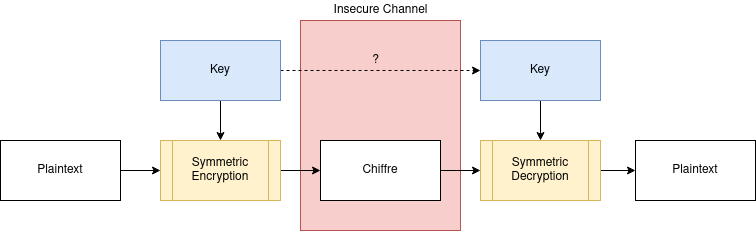
\includegraphics[width=0.8\textwidth]{background/symmetric_encryption}
  \caption[Symmetric encryption scheme]{Simple symmetric encryption scheme: Encryption and decryption algorithm use the same key.} \label{fig:symmetric-encryption}
\end{figure}

In the following, the symmetric decryption and encryption is expressed in a more formal way. The common key \textit{k} is used for encryption (\textit{Enc}) and decryption (\textit{Dec}), \textit{p} is the plaintext and \textit{c} is the ciphertext:

\begin{align*}
Enc(p, k) = c\\
Dec(c, k) = p
\end{align*}

\subsubsection{Asymmetric Cryptography}

In asymmetric cryptography each participating subject needs to generate a key pair, that consist of a private key and a public key. As mentioned above, the public key needs to be public (e.g. stored in a public database or a public key server). The private key is only known to the subject and needs to be kept secret.
\autoref{fig:asymmetric-encryption} shows an example for asymmetric encryption. Assume Alice wants to send encrypted data to Bob. Therefore, Bob created a key pair and published his public key. Alice requests Bobs public key (e.g. from a public database) and uses it to encrypt the data. Once Bob received the ciphertext, he uses his secret private key for decryption in order to retrieve the original  plaintext.

\begin{figure}[htpb]
  \centering
  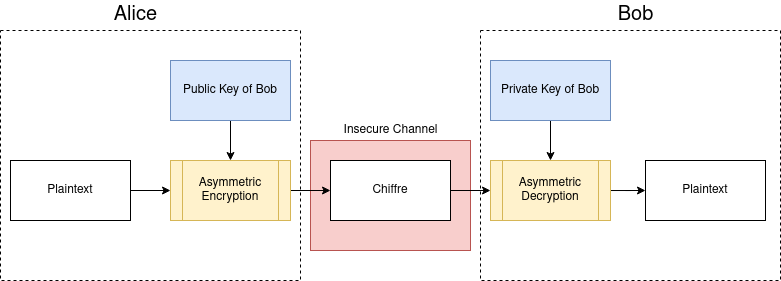
\includegraphics[width=0.8\textwidth]{background/asymmetric_encryption}
  \caption[Asymmetric encryption scheme]{Asymmetric encryption scheme: Encryption and decryption algorithm use different keys.} \label{fig:asymmetric-encryption}
\end{figure}

To formalize this procedure, again assume \textit{p} as plaintext and \textit{c} as ciphertext. The generated key pair of Bob consists of a private key for decryption ($d_{Bob}$) and a public key for encryption ($e_{Bob}$).

\begin{align*}
Enc(p, e_{Bob}) = c\\
Dec(c, d_{Bob}) = p
\end{align*}
\\
In contrast to the symmetric encryption, no secret key needs to be exchanged. However, the encryption and decryption of data using asymmetric encryption require intensive mathematical computations. Hence, the encryption of big sets of data using asymmetric encryption is not efficient.
One the other hand, symmetric encryption algorithms are usually based on simple operations, such as bit shifting or XOR. This can be implemented efficiently in software and hardware. Thus, the practical relevance of symmetric encryption is enormous.~\parencite{ITSicherheit}
\\
As stated above, securely exchanged keys are a precondition for the use of efficient symmetric encryption schemes. In order to exchange arbitrary keys securely, different key exchange protocols are available.

\section{Key Exchange}
\subsection{Diffie-Hellman Key-Exchange}

The Diffie-Hellman key exchange was introduced by Whitfield Diffie and Martin Hellman in 1976 ~\parencite{diffie1976new}. The resulting shared key of the protocol is calculated decentralized and is never transported over an insecure channel.

\subsubsection{Protocol}
The classical Diffie-Hellman key exchange assumes, that Alice and Bobs want to create a shared secret key. Therefore, they agree on a big prime $p$ and $g$, which is a primitive root modulo $p$. \footnote{The primitive root modulo p is a generator element for the set S = $\{1, 2, ... , p-1\}$.~\parencite{ITSicherheit}} Both, $p$ and $g$ are not secret and may be known to the public. \parencite{watjen2018kryptographie}

\begin{enumerate}
\item Alice choses a random $a \in \{1, 2, ... , p-2\}$ as private key. 
\item Alice calculates the public key $A = g^a mod p$.
\item Bob choses a random $b \in \{1, 2, ... , p-2\}$ as private key. 
\item Bob calculates the public key $B = g^b mod p$.
\item Alice and Bob exchange their public keys $A$ and $B$.
\item Alice calculates: 
\begin{equation}
\begin{split}
k_{AB} & = B^a mod p \\
 & = (g^b mod p)^a mod p \\
 & = g^{a b} mod p
\end{split}
\end{equation}
\item Bob calculates: 
\begin{equation}
\begin{split}
k_{AB} & = A^b mod p \\
 & = (g^a mod p)^b mod p \\
 & = g^{b a} mod p \\
 & = g^{a b} mod p
\end{split}
\end{equation}
\item Alice and Bob created the shared secret $k_{AB}$. Note that only the public keys of Alice and Bob were send over an insecure channel. The generated secret was calculated decentralized by Alice and Bob.
\end{enumerate}

\subsubsection{Security}
If an attacker wants to compute $k_{AB}$, it needs to compute the private keys $A$ and $B$ of Alice and Bob. Since only the public keys are exchanged, the attacker needs to compute:
\begin{equation*}
\begin{split}
b &= log_g\:B\:mod\;p\\ 
a &= log_g\:A\:mod\;p
\end{split}
\end{equation*}
\\
Hence, the security of the classical Diffie-Hellman key exchange is based on the discrete logarithm problem (see \ref{discrete_log_problem}). When using ephemeral key pairs, the Diffie-Hellman key exchange may be used as efficient perfect forward secrecy (PFS) protocol. ~\parencite{ITSicherheit}
\\
In modern cryptography elliptic curves are often used to increase the security of the Diffie-Hellman key exchange (ECDH). The participants have to agree on an elliptic curve and and point $P$ on the elliptic curve. The computations to generate the shared secret $k_{AB}$ follow the same principles, but obviously they are adopted to work on elliptic curves. The advantage of ECDH is the increased security strength while using the same key length than the classical Diffie-Hellman protocol. ~\parencite{ITSicherheit}
\\
Note that the introduced protocol does not authorize the participating subjects and does not guarantee integrity. Thus, this simple protocol may be exploited by a Man-In-The-Middle attack. A more advanced protocol using certificates and signed messaged could be implemented, to guarantee authentication and integrity. ~\parencite{ITSicherheit}

\subsection{Key Encapsulation}

Key encapsulation methods (KEM) transmit a previously generated symmetric key. KEMs usually use asymmetric key pairs in order to encrypt the generated symmetric key. In the following the concept is shown by the RSA based PKCS \#1 v1.5 algorithm, which uses RSA key pairs to transmit a shared secret from Alice to Bob \parencite{rsakem}:

\begin{enumerate}
\item Bob generates a RSA key pair with the public key $e_{Bob}$ and the private key $d_{Bob}$ and transmits the public key to Alice.
\item Alice generates a random secret key $k_{AB}$:
\begin{equation*}
k_{AB} = random()
\end{equation*}
\item Alice maps this secret to an integer $m$, using a well-defined mapping function $h$:
\begin{equation*}
m = h(k_{AB})
\end{equation*}
\item Alice encrypts $m$ with Bobs public key using the RSA encryption algorithm and transmits $c$ to Bob.
\begin{equation*}
c = RSA_{enc}(m, e_{Bob})
\end{equation*}
\item Bob decrypts the received ciphertext $s$ to obtain the integer $m$:
\begin{equation*}
m = RSA_{dec}(c, d_{Bob})
\end{equation*}
\item Finally bob uses the inverse mapping function $h^{-1}$ to retrieve the shared secret:
\begin{equation*}
k_{AB} = h^{-1}(m1)
\end{equation*}

\end{enumerate}

\subsection{Differences}
TODO: differences betweent kem and kex (decentralized, pfs?), discrete log vs factorization

\section{Post-Quantum Cryptography}

In the following a \textit{classical computer} refers to a non-quantum computer, which can be simulated by a deterministic Turing machine. In contrast to \textit{classical computer} the term \textit{quantum computer} describes a machine, which uses quantum mechanical phenomena to perform computations. It is important to note, that quantum computers can simulate classical computers. In addition, classical computer are able to simulate quantum computers with exponential time overhead. Thus, classical and quantum computations can calculate the same class of functions. However, quantum computers enable operations, that allow much faster computation.
 \parencite{nielsen2002quantum} \\\\
The security of modern asymmetric cryptographic primitives is usually based on difficult number theoretic problems, e.g. the discrete logarithm problem (DH, ECDH) or the factorization problem (RSA). \parencite{chen2016report} These problems are theoretically solvable, but the computation of a result on classical computer claims an impractical amount of resources. In 2019, scientists solved the factorization problem for a 240 digit integer in about 900 core-years on a classical computer (one core year means running a CPU for a full year). \parencite{boudot2795} In the following the discrete logarithm problem and the factorization problem are described.

\subsubsection{Discrete Logarithm Problem} \label{discrete_log_problem}
The discrete logarithm problem is the following challenge \parencite{beutelspacher2010diskrete}: Given a prim $p$ and two integers $g$ and $y$. Find an integer $x$, such that
\begin{equation*}
\begin{split}
&y = g^x mod p \\
\iff &x = log_g\;y\:mod p
\end{split}
\end{equation*}
Until today, it is not known if a classical computer is able to compute the general discrete logarithm problem in polynomial time. Thus, the discrete logarithm problem is considered to be difficult so solve for classical computers.  \parencite{beutelspacher2010diskrete} This assumption makes the discrete logarithm problem an attractive basis for DSA, ElGamal, the classical Diffie-Hellman protocol, and for the elliptic curve Diffie-Hellman (ECDH).

\subsubsection{Factorization Problem}

Given two large primes p and q, it is easy to compute the the product of them:
\begin{equation*}
n = p \star q
\end{equation*}
For a given $n$, however, it is difficult to find the prime factors $p$ and $q$. The computation of the prime factorization for a given integer $n$ is called the factorization problem. \parencite{ITSicherheit} For large numbers n no efficient algorithm for classical computers is known to solve this problem. \parencite{ITSicherheit} The most famous cryptographic protocol, which builds upon the hardness of the factorization problem is RSA.

\subsection{Impact of Quantum Computers on Cryptography}

As stated above, quantum computers enable new operations which speed up certain algorithms. Two quantum algorithms which have enormous consequences on modern cryptography are \textit{Shor's algorithm} and \textit{Grover's algorithm}. \parencite{nielsen2002quantum}
\\\\
Peter Shor published \textit{"Algorithms for quantum computation: discrete logarithms and factoring"} in 1994 \parencite{shor1994algorithms}, where he demonstrated that the factorization problem and the discrete logarithm problem can be solved in polynomial time on quantum computers. Both problems are the basis of many public-key systems (RSA, DH, ECDH, ...), which are used intensively in modern communication systems. Hence, a quantum computer running \textit{Shor's algorithm} would qualify the assumption of most asymmetric encryption schemes and thus break their security.
\\\\
The second algorithm having impact on computer security was published by Lov Grover in 1996 (\textit{"A fast quantum mechanical algorithm for database search"}, \parencite{grover1996fast}) - namely \textit{Grover's algorithm}. The algorithms solves the problem of finding an element $y$ in a set $s$ (e.g. a database) where $|s| = N$. On a classical computer an algorithm solving the problem runs in $\mathcal{O}(N)$, however \textit{Grover's algorithm} has complexity $\mathcal{O}(\sqrt{N})$. \parencite{nielsen2002quantum}\\
In contrast to public-key systems, which relay on hard mathematical problems, symmetric encryption schemes relay on the secrecy of a randomly generated key. 
Thus, to break symmetric encryption one need to perform a brute-force attack on the symmetric key. Using \textit{Grover's algorithm} offers a square root speed up on classical brute force attacks. Assume a randomly generated $n$-bit key. A classical brute force algorithm lies in $\mathcal{O}(2^n)$, which is considered to be safe for a big $n$ (e.g. $n$=128). \textit{Grover's algorithm} speeds up this attack to $\mathcal{O}(\sqrt{2^n})$ = $\mathcal{O}(2^{n/2})$. \parencite{mavroeidis2018impact} However, the complexity is still exponential and with a growing key sizes $n$ the security can be increased. Thus, \textit{Grover's algorithm} forces symmetric encryption schemes to increase their used key size in order to stay secure.
\\\\
To sum up, quantum computers make use of quantum mechanical phenomena in order to solve mathematical problems, which are assumed to be difficult for modern computers. As a result quantum computers might break many algorithms of modern asymmetric cryptography and enforce increased key sizes for symmetric encryption schemes. The following table form the NIST \textit{"Report on Post-Quantum Cryptography"} (\parencite{chen2016report}) shows the impact of quantum computers on modern encryption schemes:

\begin{table}[htpb]
  \caption[Impact of quantum computers on encryption schemes]{Impact of quantum computers on encryption schemes}\label{tab:impact}
  \centering
  \begin{tabular}{|p{3cm}|p{3cm}|p{3cm}|p{5cm}|}
	\hline
    \rowcolor{lightgray!50}
      \textbf{Cryptographic} \newline \textbf{algorithm} & \textbf{Type} & \textbf{Purpose} & \textbf{Impact from} \newline \textbf{ quantum computer} \\
	\hline
      AES & Symmetric key & Encryption & Larger key sizes needed \\
    \hline
      SHA & --- & Hash functions & Larger output needed \\
    \hline
      RSA & Public key & Signatures,\newline key establishment & No longer secure \\
	\hline      
      DSA & Publiy key & Signatures,\newline key exchange & No longer secure \\
    \hline
      ECDH, ECDSA & Public key & Signatures,\newline key exchange & No longer secure \\
    \hline
  \end{tabular}
\end{table}
\subsection{Classes of Post-Quantum Cryptography}
\subsection{Isogeny-based Cryptography (SIDH)}
